\begin{figure}[!htbp]
\centering
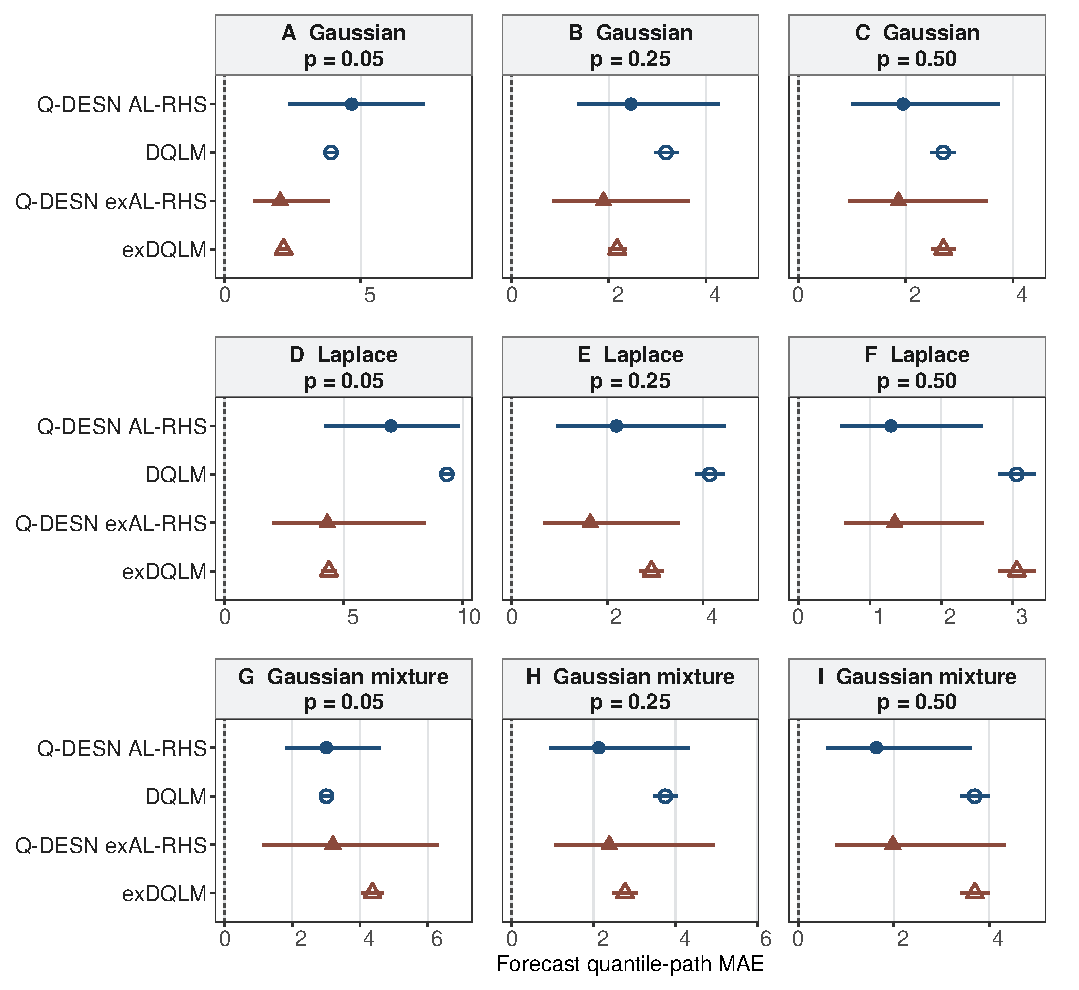
\includegraphics[width=0.98\textwidth]{figures/independent_simulation/independent_train500_eval300_mcmc_forecast_mae_v1.pdf}
\caption{MCMC forecast quantile-path MAE over the first 300 evaluation targets (10 origins). Points and equal-tailed 95\% intervals summarize the draw-wise criterion averaged over scored pairs; lower is better. Navy circles identify \(\AL\) models and muted-brick triangles \(\exAL\) models; filled symbols denote Q--DESN and open symbols their dynamic linear comparators. Panels A--I identify the observation-error family and probability level. The dashed line marks exact recovery of the state-conditional quantile path. Corresponding panels in the 500-target sensitivity figure use the same horizontal limits. The supplement documents criterion-specific selection and model-specific forecast-draw dependence.}
\figalt{Nine panels compare four models using mean forecast quantile-path MAE and 95 percent intervals over 300 scored targets.}
\label{fig:simulation-500obs-mcmc-forecast-mae-intervals}
\end{figure}
